\item Assume that protons and neutrons have equal masses. Mass of a nucleon is \(1.6 \times 10^{-27}\) kg and radius of nucleus is \(1.5 \times 10^{-15} A^{1/3}\) m. The approximate ratio of the nuclear density and water density is \(n \times 10^{13}\). The value of \(n\) is \underline{\hspace{2.5cm}}.
    \begin{center}
        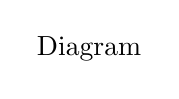
\begin{tikzpicture}
            \node at (0, 0) {Diagram};
        \end{tikzpicture}
    \end{center}